

\subsection{Estimação do modelo BEKK.}\label{estimacao-do-modelo-bekk.}

Na seção anterior realizou-se a estimação do modelo de vetor de correção
de erros para a obtenção do resíduo livre do co-movimento entre as
médias. Porém, ao usarmos 4 defasagens para o modelo VAR, e
consequentemente 3 defasagens para o modelo VEC, os resíduos do modelo
VEC ainda apresentaram correlação. Já que o método de estimação BEKK
proposto por \citeonline{engle_multivariate_1995} supõe que os dados sejam não
correlacionados e isso não ocorreu após a estimação do modelo VEC (os
resíduos permaneceram correlacionados) foi realizado o mesmo
procedimento anterior, mas escolhendo diferentes defasagens para o
modelo VAR. Constatamos que usando o número máximo de desafagens (7),
indicado pelo critério AIC, os resíduos do modelo VEC estimado
posteriormente não apresentam correlação serial até a vigésima
defasagem. Portanto o modelo BEKK será estimado usando os resíduos do
modelo VEC com 6 defasagens.

Com este novo número de defasagens escolhido, assim como no caso
anterior, identificamos um único vetor de cointegração (1, -0,125,
-0,358). Para sintetizar as correlações dos resíduos do modelo VEC(7),
plotamos os valores-p do teste de Ljung-Box realizado para estes
resíduos.

\begin{figure}[htbp]
\centering
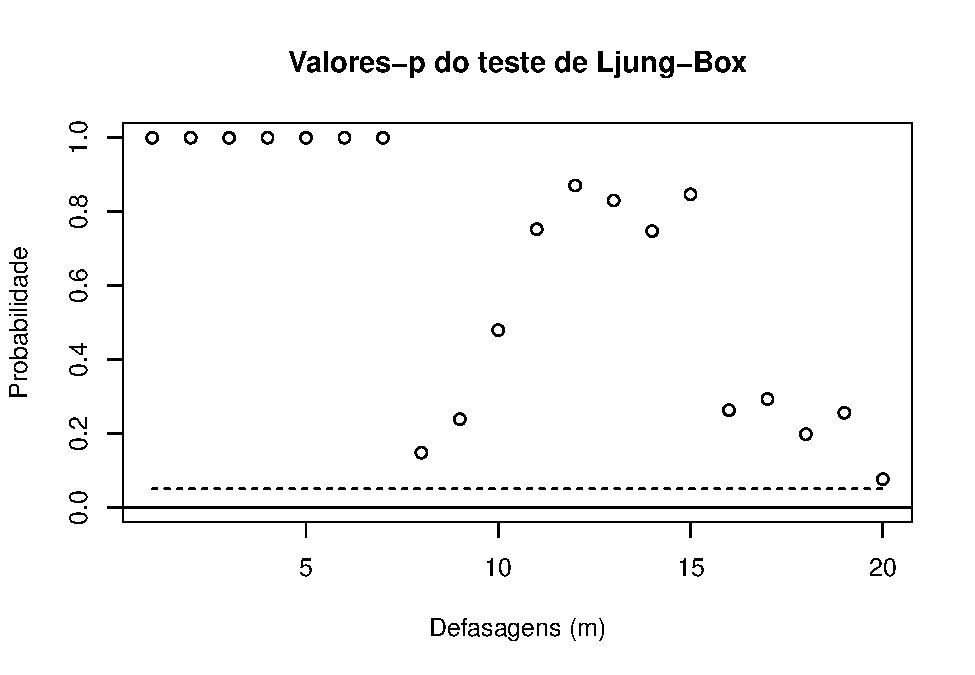
\includegraphics{mq2 test-1.pdf}
\caption{Plotagem dos valores-p das defasagens do teste multivariado de
correlação Ljung-Box.}
\end{figure}

Como podemos observar, todas os valores-p estão são maiores que 5\%
(linha tracejada). Portanto para estas defasagens não se rejeita a
hipótese nula de ausência de autocorrelação e correlação entre as
variáveis. Uma vez identificado que os resíduos não são correlacionados,
como impõe o modelo BEKK, podemos seguir adiante nas estimações.

Estimação do modelo BEKK.

\begin{verbatim}
## Initial estimates:  -3.370388e-06 9.138433e-05 -2.972673e-05 0.008118471 0.0004654883 0.0005525955 0.008979964 0.0007634438 0.006105187 0.1 0.02 0.02 0.02 0.1 0.02 0.02 0.02 0.1 0.8 0.02 0.02 0.02 0.8 0.02 0.02 0.02 0.8 
## Lower limits:  -3.370388e-05 -0.0009138433 -0.0002972673 0.001623694 9.309765e-05 0.0001105191 0.001795993 0.0001526888 0.001221037 1e-06 -0.5 -0.5 -0.5 1e-06 -0.5 -0.5 -0.5 1e-06 1e-06 -0.5 -0.5 -0.5 1e-06 -0.5 -0.5 -0.5 1e-06 
## Upper limits:  3.370388e-05 0.0009138433 0.0002972673 0.008930318 0.0005120371 0.000607855 0.00987796 0.0008397882 0.006715706 0.999999 0.5 0.5 0.5 0.999999 0.5 0.5 0.5 0.999999 0.999999 0.5 0.5 0.5 0.999999 0.5 0.5 0.5 0.999999 
## 
## Coefficient(s):
##                Estimate   Std. Error  t value   Pr(>|t|)    
## mu1.etanol -2.84925e-06  2.47352e-04 -0.01152  0.9908093    
## mu2.acucar  9.14653e-05  3.29909e-04  0.27724  0.7815925    
## mu3.soja   -3.01570e-05  2.05733e-04 -0.14658  0.8834611    
## A011        7.18811e-03           NA       NA         NA    
## A021        4.24346e-04  3.56933e-04  1.18887  0.2344910    
## A031        4.97986e-04  1.92549e-04  2.58629  0.0097017 ** 
## A022        8.14837e-03           NA       NA         NA    
## A032        7.05890e-04           NA       NA         NA    
## A033        4.89427e-03           NA       NA         NA    
## A11         9.99998e-02  4.68451e-02  2.13469  0.0327862 *  
## A21         1.99998e-02  3.27585e-02  0.61052  0.5415152    
## A31         1.99996e-02  2.29792e-02  0.87034  0.3841162    
## A12         1.99997e-02  2.67969e-02  0.74634  0.4554604    
## A22         9.99993e-02  3.03239e-02  3.29770  0.0009748 ***
## A32         1.99997e-02  1.91742e-02  1.04305  0.2969232    
## A13         1.99998e-02  3.69084e-02  0.54188  0.5879025    
## A23         1.99999e-02  4.11480e-02  0.48605  0.6269333    
## A33         9.99995e-02  3.83827e-02  2.60533  0.0091786 ** 
## B11         7.99983e-01  8.83433e-03 90.55387 < 2.22e-16 ***
## B21         1.99973e-02  1.39432e-02  1.43420  0.1515161    
## B31         1.99956e-02  5.13848e-03  3.89134 9.9692e-05 ***
## B12         1.99964e-02  1.19954e-02  1.66700  0.0955135 .  
## B22         7.99983e-01           NA       NA         NA    
## B32         1.99949e-02  3.52939e-03  5.66526 1.4680e-08 ***
## B13         1.99974e-02  1.26003e-02  1.58705  0.1125005    
## B23         1.99977e-02  1.28828e-02  1.55228  0.1205947    
## B33         7.99982e-01           NA       NA         NA    
## ---
## Signif. codes:  0 '***' 0.001 '**' 0.01 '*' 0.05 '.' 0.1 ' ' 1
\end{verbatim}

Todos os coeficientes foram positivos, o que era esperado pois o modelo
BEKK implica que a matriz de variância e covariância seja positiva
definida. Poucos coeficientes estimados se mostraram significantes, o
que significa dizer que as volatilidades passadas não têm grande impacto
sobre sua própria volatilidade corrente e sobre as volatilidades dos
preços das outras \emph{commodities}. Os efeitos que se mostraram
significativos com nível de significância de 5\% foram: Com respeito ao
impacto médio da volatilidade (matriz de covariância incondicional)
apenas o soja é impactado pelo etanol, os demais efeitos não são
significativos. Em relação aos efeitos ARCH, as três \emph{commodities}
apresentaram sofrer influência de suas próprias inovações e nenhum
efeito cruzado se mostrou significativo. Agora com respeito ao
componente autorregressivo da matriz da covariâncias (efeito GARCH),
somente o etanol se mostrou significativo com respeito à efeitos
próprios. Os efeitos cruzados GARCH ocorreram para o soja sendo
impactado tanto pelo etanol quanto pelo açúcar. Ao que sugere o modelo
BEKK estimado, somente o soja sofre impactos significativos das outras
\emph{commodities}, enquanto o açúcar e o etanol sofrem influência
apenas de suas próprias inovações e volatilidades. Outra conclusão que
se pode tirar do modelo, é que o etanol possui um efeito mais forte
sobre o soja do que o açúcar, pois o etanol afeta o soja por meio da
matriz de covariância condicional e incondicional, enquanto o açúcar
impacta o soja apenas pela matriz de covariâncias condicional.


